\chapter{Interface gráfica}
\label{interface}

A interface gráfica é responsável pela interação com o usuário.

Uma janela, ``Program'', contém um caixa de texto multilinha, onde
o usuário deve escrever o programa.
Um botão, ``Compile'', compila o texto escrito.
A resposta do compilador será ``Status: OK'' para um programa compilado 
corretamente, ou ``Status: ...'' com uma mensagem de erro, indicando a
linha e a coluna correspondentes.
Dois controles deslizantes definem o tamanho, em pixels, da janela
de visualização 3D(``Frame size'') e do Geodesic Tracing(``Geo Size'').
Um botão, ``Open Texture'', serve para carregar uma imagem local,
com o nome informado à caixa de texto justaposta.

A figura \ref{img:program} ilustra a janela ``Program''.

\begin{figure}[!ht]
    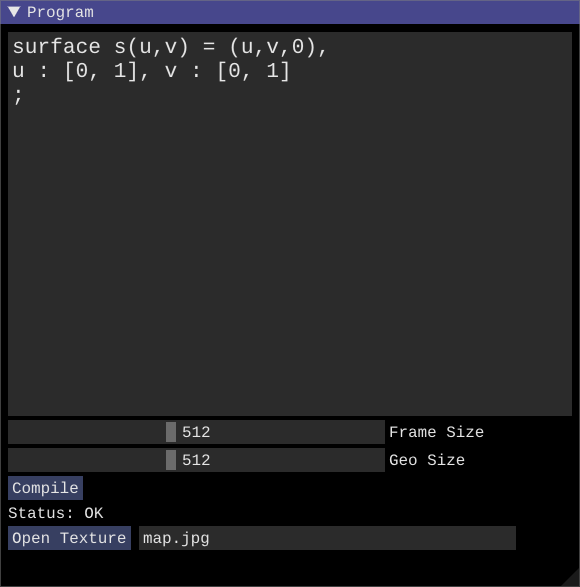
\includegraphics[width=\linewidth]{program.png}
    \caption{Janela ``Program''}
    \label{img:program}
\end{figure}

Quando o programa é compilado corretamente, duas janelas extras são exibidas.

A janela ``Settings'' controla algumas propriedades dos objetos.
Para os parâmetros, um controle deslizante é criado, com a opção ``Animate''.
Quando ativado, o parâmetro é controlado pelo tempo,
crescendo uma unidade por segundo.
Quando o limite superior do parâmetro é atingido,
o valor volta para o limite inferior.

Para cada objeto desenhável é possível escolher uma cor.

Para uma superfície, os componentes RGB da textura
são multiplicadas pelos componentes RGB da cor escolhida.
A cor branca deixa a textura inalterada,
e preto deixa a textura completamente preta.
Além disso, é possível escolher uma textura previamente carregada para
uma superfície. A textura padrão é a textura local de nome ``default.jpg''.

A velocidade da câmera é controlada por ``Camera speed''.
Esse valor afeta as câmeras das janelas ``3D view'' e de ``Geodesic Tracing''.

A figura \ref{img:settings} ilustra a janela ``Settings''.

\begin{figure}[!ht]
    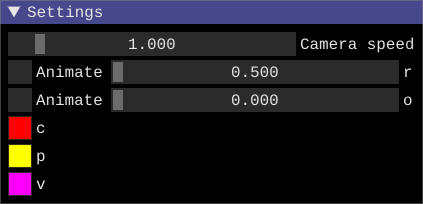
\includegraphics[width=\linewidth]{settings.png}
    \caption{Janela ``Settings''}
    \label{img:settings}
\end{figure}

A janela ``3D View'' exibe os objetos desenháveis no espaço 3d.
A câmera pode ser controlada da seguinte forma:

\begin{centering}
\begin{tabularx}{\textwidth}{||c|X||}
    \hline
    \texttt{W} & move a câmera para frente \\
    \hline
    \texttt{S} & move a câmera para trás \\
    \hline
    \texttt{A} & move a câmera para a esquerda \\
    \hline
    \texttt{D} & move a câmera para a direita \\
    \hline
    \texttt{Q} & move a câmera para cima (absoluto) \\
    \hline
    \texttt{E} & move a câmera para baixo (absoluto) \\
    \hline
    \texttt{Click \& move} & gira a câmera conforme o movimento do mouse \\
    \hline
\end{tabularx}
\end{centering}

Para uma superfície ``X'', a janela ``Geodesic Tracing - X'' é exibida.
A janela exibe a visualização do geodesic tracing.

A câmera pode ser controlada da seguinte forma:

\begin{centering}
\begin{tabularx}{\textwidth}{||c|X||}
    \hline
    \texttt{W} & move a câmera para frente \\ 
    \hline
    \texttt{S} & move a câmera para trás \\
    \hline
    \texttt{A} & move a câmera para a esquerda \\
    \hline
    \texttt{D} & move a câmera para a direita \\
    \hline
    \texttt{Q} & gira a câmera no sentido anti-horário \\
    \hline
    \texttt{E} & gira a câmera no sentido horário \\
    \hline
    \texttt{Z} & zoom in \\
    \hline
    \texttt{X} & zoom out \\
    \hline
    \texttt{Click \& move} & move a câmera conforme o movimento do mouse \\
    \hline
\end{tabularx}
\end{centering}